\subsection{System Design}

The feedback of the test part of the system will consist of a compass plot, where the output will be based on either the regression based control scheme alone or a combined model with classification included as well.

\begin{figure}[H]                                        
	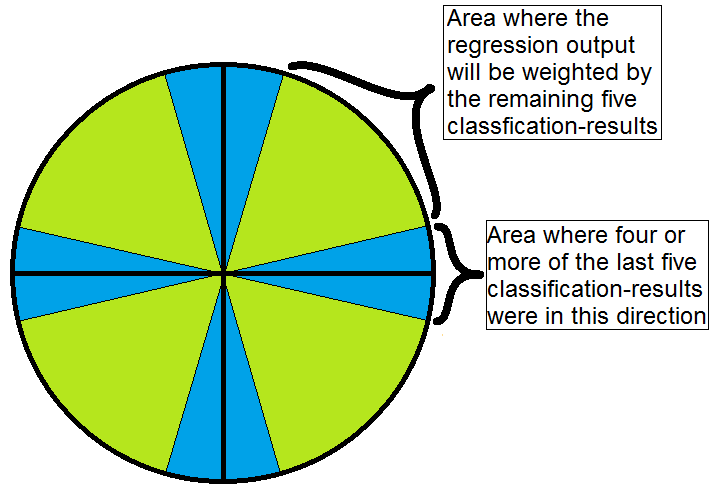
\includegraphics[width=0.8\textwidth]{figures/controlSuggestion} 
	\caption{Suggestion on the areas where multiple DOF's (green) and a single DOF (blue) will be activated in the compass plot inside the GUI with a control scheme based on both classification and regression}
	\label{fig:controlSuggestion} 
\end{figure}  

When testing the combination of regression and classification, the system will be designed with the regression result as the main output while the classification results will be used as weights to determine if the subject intends to perform a single movement or a combination of multiple movements. The system will perform a single movement if four of the previous five classification outputs were the same movement. This means that there will be a certain area where the output will be in a single direction, as shown with blue on \figref{fig:controlSuggestion}. Combining the two types of control should give the user a possibility to activate a single DOF proportional movement without being extremely precise.

In cases where the subject intends to activate multiple DOF's at the same time in the green areas of \figref{fig:controlSuggestion}, the previous five classification results will be used to weight the regression outputs. An example of this could be three extensions and two radial deviations within the five most recent classifier results, where the extension regression output will be weighted with $ \dfrac{3}{5} $ and the radial deviation will have a weight of $ \dfrac{2}{5} $. This implementation should give the subject a possibility of activating multiple DOF's proportionally at the same time. 

The output of the regression based control scheme will be translated directly to the compass plot, where it will be used to reach targets in the test. This means that the subjects will have to be more precise when trying to activate a single DOF, as there are no areas where the classifier will force the output to be a single DOF.